\documentclass[12pt]{article}
\usepackage{geometry}
\geometry{letterpaper, left=22.5mm, right=22.5mm, top=30mm, bottom=30mm}
\geometry{letterpaper}
\usepackage{amsmath}
\usepackage{amssymb}
\usepackage{enumitem}
\usepackage{fancyhdr}
\usepackage{framed}
\usepackage{tikz}
\usepackage{mathpazo}
%\usepackage{charter}
%\usepackage{newcent}
\usepackage{indentfirst}
\usepackage{booktabs}
\usepackage{graphicx}
\usepackage{float}
\usepackage{makecell}
\usepackage{xcolor}
\usepackage{mdframed}
\usetikzlibrary{trees}
\pagestyle{fancy}
\usepackage{amsthm}
\theoremstyle{definition}
\newtheorem{definition}{Definition}[section]
\theoremstyle{property}
\newtheorem{property}{Property}[section]
\theoremstyle{assumption}
\newtheorem{assumption}{Assumption}[section]
\theoremstyle{example}
\newtheorem{example}{Example}[section]
\theoremstyle{comment}
\newtheorem{comment}{Comment}[section]
\newtheorem{theorem}{Theorem}[section]
\newtheorem{corollary}{Corollary}[theorem]
\newtheorem{lemma}[theorem]{Lemma}
\usepackage{lastpage}
\usepackage{wrapfig}
\usepackage{hyperref}
\usepackage{subcaption}
\usepackage{setspace}
\hypersetup{
colorlinks=true,
linkcolor=black,
filecolor=green, 
urlcolor=blue,
}
\newcommand{\ROM}[1]
    {\MakeUppercase{\romannumeral #1}}
\fancyhead[L]{Econometrics \ROM{2}: Recitation 2}%change each reci
\fancyhead[R]{Spring 2022}
\fancyfoot[C]{\thepage \hspace{1pt} / \pageref{LastPage}}

\fancypagestyle{firstpage}{%
\fancyhf{}%
\renewcommand{\headrulewidth}{0mm}%
  \fancyfoot[C]{\thepage \hspace{1pt} / \pageref{LastPage}}
}
%change title each rec
\title{Introduction to Econometrics \ROM{2}: Recitation 3}

\begin{document}
\linespread{1.25}
\onehalfspacing

\author{Seung-hun Lee\footnote{Contact me at \href{mailto:sl4436@columbia.edu}{sl4436@columbia.edu} if you spot any errors or have suggestions on improving this note.}}
\date{February 7th, 2022}
\maketitle
\thispagestyle{firstpage}

%%%%%%%%%%%%%%%%%%
\section{Various tests in IV and GMM framework}
\begin{mdframed}[backgroundcolor=yellow!5] 
\begin{comment}[Wald vs Lagrangian Multiplier vs Likelihod Ratio (Engle, 1984\footnote{Engle, R. (1984) `Wald, Likelihood Ratio, and Lagrange Multiplier Tests in Econometrics. In Z Grillches, M. D. Intrilligator (Ed.), Chapter 13 of the \textit{Handbook of Econometrics} Volume 11, 775-826})] 
\par
Suppose we have the data $y$, parameter of interest $\beta$ and the log likelihood function $L(y,\beta)$. The hypothesis we want to check is
\[
H_0:\beta=\beta_0 \ \text{vs} \ H_1: \beta\neq\beta_0
\]
\begin{itemize}
\item Wald: This is a test based on unconstrained regression in the sense that it tests the composite alternative hypothesis against the null. The idea is to accept the null when th e estimated value of $\beta$ is reasonably close to $\beta_0$. The typical test statistics is
\[
t_{W} = (\hat{\beta}-\beta_0)'(var(\hat{\beta}))^{-1}(\hat{\beta}-\beta_0) \sim \chi^2_{\dim{(\beta)}}
\]
\item LM: This is based on the constrained minimization problem of the likelihood function. We impose the null hypothesis with the following constrained optimization problem
\[
L(y,\beta)-\lambda'[\beta-\beta_0]
\]
with the first order conditions
\begin{itemize}
\item With respect to $\beta$:  $\frac{\partial L}{\partial \beta} = \lambda$
\item With respect to $\lambda$: $\beta=\beta_0$
\end{itemize}
By complementary slackness conditions, we would have $\lambda\geq0$ and $\lambda=0$ if the constraint is not binding. If the shadow price is high (high $\lambda=s(y,\beta_0)$), then we would reject the constraint. Typically, the test statistics used has this form:
\[
t_{LM} = s(y,\beta_0)'(var(s))^{-1}s(y,\beta_0) \sim \chi^2_{\dim(\beta)}
\]
\item LR: This is based on the difference between the maximum of the likelihood under the null vs under the alternative. Typically, the test statistics have the following form
\[
t_{LR} = -2[L(y,\beta_0)-L(y,\hat{\beta})]\sim \chi^2_{\dim(\beta)}
\] 
\end{itemize}
Takeaway is that all three have the same asymptotic distribution. However, the computational requirement is different. We should check whether we are imposing the null hypothesis when the test statistics are created, or whether we are just comparing the distance between the null and the unconstrained estimator. 
\par
Here is a picture summarizing the difference between the three
\begin{figure}[H]
\begin{center}
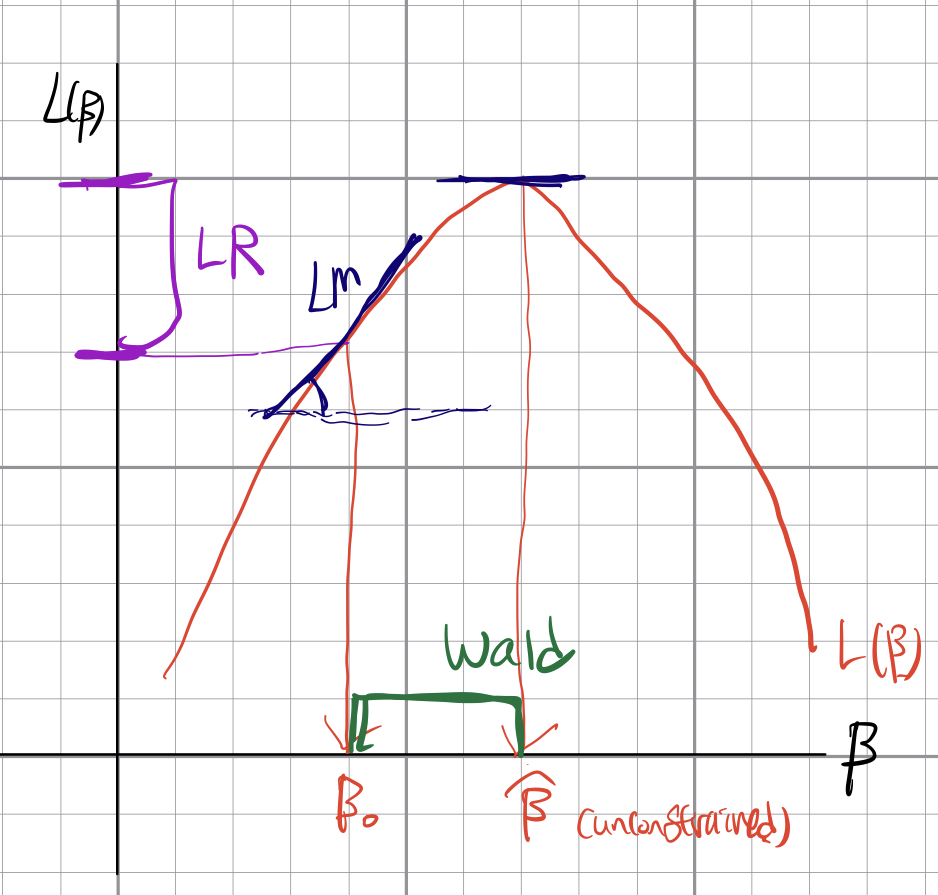
\includegraphics[width=0.5\textwidth, keepaspectratio]{3test.jpeg}
\caption{Wald vs LM vs LR}
\end{center}
\end{figure}
\end{comment}
\end{mdframed}
\subsection{J test for overidentifying restrictions}
Consider the following setup
\[
y_i = x_i'\beta+e_i, \ (\dim(x_i)=k<\dim(z_i)=l) 
\]
where we have an overidentified model, with number of instruments being larger than endogenous variables. We can test for the validity of the instruments by testing $H_0: E(z_ie_i)=0$ vs. $H_1: E(z_ie_i)\neq0$. 
\par
I will cover two setups for this test
\subsubsection{Hansen's test: Using the GMM framework}
In this setup, we are testing for the hypothesis 
\[
H_0: E[g(w_i,\beta)]=0 \ \text{vs. } H_1: E[g(w_i,\beta)]\neq0
\]
where $g(w_i,\beta)=z_ie_i$. One natural candidate statistics to assess this hypothesis is $\bar{g}(\beta)=\frac{1}{n}\sum_{i=1}^n z_ie_i$, since this converges in probability to $E[z_ie_i]$. The test statistics that comes out from this is the GMM criterion function $J(\beta)=n\bar{g}(\beta)'\widehat{\Omega}^{-1}\bar{g}(\beta)$. The asymptotic distribution of $J(\beta)$ can be analyzed as follows: Note that $\sqrt{n}\bar{g}(\beta)\xrightarrow{d}N(0,\Omega)$ where $\Omega\in\mathbb{R}^{l\times l}$. $J(\beta)$ can be rewritten as
\[
\begin{aligned}
J(\beta)&= \underbrace{\left(\sqrt{n}\bar{g}(\beta) \right)'}_{\xrightarrow{d}N(0,\Omega)} \widehat{\Omega}^{-1}\underbrace{\left(\sqrt{n}\bar{g}(\beta) \right)}_{\xrightarrow{d}N(0,\Omega)}\\
&\xrightarrow{d} \chi^2_l
\end{aligned}
\] \par
However, when we are implementing this in the practice, we need an estimate of $e_i$. The natural candidate is to use the residuals we get after a GMM estimation, $\hat{e}_i = y_i-x_i'\hat{\beta}_{GMM}$. Once we obtain the residuals, we get the usable test statistics $J(\hat{\beta}_{GMM})$, whose asymptotic distribution is now $\chi_{l-k}^2$. The reason is that in obtaining the residuals, we have estimated $k$ parameters ($\hat{\beta}_{GMM}$). Thus, the final test statistic and its distribution under the null is
\[
J=J(\hat{\beta}_{GMM})\xrightarrow{d} \chi_{l-k}^2
\] 
In terms of rejecting the null or not in a test with significance level $\alpha$, we compare the $J$ value with the critical value $\chi_{l-k, \alpha}^2$ where $\Pr(\chi^2\geq\chi_{l-k, \alpha}^2) = \alpha$

\par
The test introduced here also tests for other issues with the specification. So this test checks exogeneity assumption and other specification related issues - misspecification, for instance (or both). Thus, large $J$ values might indicate violation of exogeneity, misspecification, or both. This implies that we can conclude that there are endogeneity in the overidentifying assumptions only if we are sure that the model used does not suffer from other specification-related problems.
\par
Unlike the Sargan test for 2SLS estimator that is introduced in the next section, this setup allows for a general heteroskedasticity. (We have not set any restrictions on $\Omega = E[z_iz_i'e_i^2]$)
\subsubsection{Sargan test}
You may think of this as a specific, restricted version of the Hansen's test. We go back to our original structural equation
\[
y_i = x_i'\beta+e_i \ (\dim(x_i)=k<\dim(z_i)=l) 
\]
where we assume $x_i$ is broken into $x_1$ and $x_2$. We assume $x_2$ is endogeous, but not $x_1$. We construct a linear projection equation by projecting $e_i$ onto $z_i$, obtaining
\[
e_i=z_i'\delta+\epsilon_i
\]
Thus, $\delta=E(z_iz_i')^{-1}E(z_ie_i)$.  Because of this, the null and alternative hypotheses can be expressed by $H_0: \delta=0$ vs. $H_1: \delta\neq0$. This leaves us with the challenge of estimating $\delta$.  Since we do not know what the true value of the error terms are, we take the following steps.
\begin{enumerate}
\item \textbf{Obtain $\hat{e}_i$}: This can be done using 2SLS estimates of $\beta$. As a result, 
\[
\hat{e}_i = y_i-x_i'\hat{\beta}_{2SLS} \implies \hat{e}=y-X\hat{\beta}_{2SLS}
\]
\item \textbf{Obtain $\hat{\delta}$}: Replace $e$ with $\hat{e}$ to get
\[
\hat{\delta} = (Z'Z)^{-1}Z'\hat{e}
\]
\item \textbf{Sargan Test}: We will assume homoskedasticity (otherwise, the test statistic does not converge to $\chi^2$ distribution). Then we make use of the following test statistic
\[
S=\hat{\delta}'(var(\hat{\delta}))^{-1}\hat{\delta}=\frac{\hat{e}'Z(Z'Z)^{-1}Z'\hat{e}}{\hat{\sigma}^2}
\]
where $\hat{\sigma}^2=\frac{1}{n}\hat{e}'\hat{e}$. Under the null, $S\xrightarrow{d}\chi_{l-k}^2$
\end{enumerate} \par
Same caution as before applies: Even if the null hypothesis is rejected, the test alone is not enough to pick up which extra instrumental variable violates the condition. It may even be the case that some other specification problem may lead to rejecting the null. 

\subsection{Testing exogeneity for a subset of instruments}
We can apply overidentification test on a (strict) subset of instruments whose validity is uncertain. To do this, we can partition $z_i$ into two sets - $z_{ai}\in\mathbb{R}^{l_a}$ and $z_{bi}\in\mathbb{R}^{l_b}$. We are uncertain about $z_{bi}$ and want to test 
\[
H_0: E(z_{bi}e_i)=0, \ \text{vs. }H_1:E(z_{bi}e_i)\neq0
\]\par
We can construct the test statistic in a following manner. First, estimate the model by the efficient GMM with only the $z_{ai}$ set of instruments and obtain the GMM criterion. This will be denoted as $J_a$. Then, estimate the model with the full set of instruments and obtain a separate GMM criterion, denoted as $J_{a,b}$. Then, create a test statistic
\[
C=J_{a,b}-J_a\xrightarrow{d}\chi^2_{l-l_a=l_b}
\]
The idea is similar to that of a distance test. If the $C$ value is low, then the moment condition for the larger set of instruments are not too different from the moment condition from the smaller (but surer) set of instruments. Then, we find a critical value $\chi_{l_b,\alpha}^2$ for a significance level $\alpha$ and reject the null hypothesis if $C>\chi_{l_b,\alpha}^2$. 
\par
There are two other ways to approach this: One is the Amemiya-Lee-Newey minimum chi-square statistic which uses auxiliary regression of the errors onto the set of instruments. Specifically, the idea is that by projecting $e_i$ onto two sets of instruments - the ones we are certain about ($z_a$) and the ones we are not ($z_b$) - we get
\[
e_i = z_{ai}'\delta_a+z_{bi}'\delta_b+u_i
\]
and test for the exogeneity of $z_b$ instruments by checking $\delta_b=0$. In practice, we obtain residuals $\hat{e}$ and run an auxiliary regression of this into the two sets of instruments and obtain estimates for $\delta_b$. The test statistics used and its distribution under the null is
\[
\hat{\delta}_b'(\text{var}(\hat{\delta}_b))^{-1}\hat{\delta}_b \sim \chi_{l_b}^2
\] \par
Another way to do this is using a Hausman test principle (further discussed in the next section). Obtain two estimates of $\beta$ - one using only the sure IVs and the other using all sets of IVs. Then, the idea is to check whether the two estimates are close to each other. 
\subsection{Hausman test: Application to endogeneity test}
Hausmann Test can be utilized as a general test of specification. It is aimed at testing the consistency of an estimator that we are uncertain about relative to an estimator that is surely consistent. The general trick is that you need two types of estimators. 
\begin{itemize}
\item $\hat{\theta}_1$: Consistent and efficient under $H_0$, inconsistent under $H_1$
\item $\hat{\theta}_2$: Consistent in either $H_0$ or $H_1$. Inefficient under $H_0$. 
\end{itemize}
Then the difference between the two estimators have the following asymptotic distribution
\[
\sqrt{n}(\hat{\theta}_1-\hat{\theta}_2) \sim N(0, \text{var}(\hat{\theta}_2-\hat{\theta}_1))
\]
and the test statistic that is used is
\[
H=(\hat{\theta}_1-\hat{\theta}_2)'(\text{var}(\hat{\theta}_2-\hat{\theta}_1))^{-1}(\hat{\theta}_1-\hat{\theta}_2)
\] \par
One possible usage is to test for exogeneity/endogeneity of the regressors. Assume that homoskedasticity is satisfied and the data generating process is
\[
y_i = x_{1i}'\beta_1 + x_{2i}'\beta_2+e_i
\]
and we are interested in checking the exogeneity of $x_{2i}$. So we test $H_0: E(x_{2i}e_i)=0$ against $H_1:E(x_{2i}e_i)\neq0$. Consider these properties of 2SLS and OLS estimators
\begin{itemize}
\item $\hat{\beta}_{OLS}$: Consistent and minimal variance under $H_0$, inconsistent under $H_1$
\item $\hat{\beta}_{2SLS}$:  Consistent in either $H_0$ or $H_1$. Inefficient under $H_0$. 
\end{itemize}
Under $H_0$, $\sqrt{n}(\hat{\beta}_{2SLS}-\hat{\beta}_{OLS})$ converges in distribution to $N(0, var(\hat{\beta}_{2SLS}-\hat{\beta}_{OLS}))$. Hausmann also shows that in $H_0$, $var(\hat{\beta}_{2SLS}-\hat{\beta}_{OLS})=var(\hat{\beta}_{2SLS})-var(\hat{\beta}_{OLS})$ holds in homoskedastic setting (you are asked to show this for a scalar case). Given this, we can write the Hausmann test statistic as 
\[
(\hat{\beta}_{2SLS}-\hat{\beta}_{OLS})'(var(\hat{\beta}_{2SLS})-var(\hat{\beta}_{OLS}))^{-1}(\hat{\beta}_{2SLS}-\hat{\beta}_{OLS})\xrightarrow{d}\chi_{k_2}^2
\]\par
One nice feature about this is that you can use Hausman test for many types of specification tests. For instance, you can use this to test whether it is justified to use random effects (as opposed to fixed effects) in the panel regression setup. 

\subsection{Using control function to test for endogeneity}
We now use a different way of testing for endogeneity that is robust to heteroskedastic errors. The idea is to use the setup from the control function to test for endogeneity. Assume the following setup
\[
\begin{aligned}
y_i &= x_{2i}'\beta_2+e_i& \ \ (E[x_{2i}e_i]\neq0) \\
x_{2i}&=z_i'\pi_2 + v_{2i}& \ \ (E[z_ie_i]=0, E[z_iv_{2i}]=0)\\
e_i &=v_{2i}'\rho + w_i&\\
y_i &= x_{2i}'\beta_2+v_{2i}\rho + w_i
\end{aligned}
\]
Since we do not know the true value of $v_{2i}$, we replace this with $\hat{v}_{2i}$ by running an OLS on the first stage regression  and then write
\[
y_i = x_{2i}'\beta_2+\hat{v}_{2i}\rho + w_i
\] \par
What we need to do is to check whether $\hat{\rho}=0$ or not. Recall that
\[
\begin{aligned}
E[x_{2i}e_i]&=E[(z_i'\pi_2 + v_{2i})e_i]\\
&=E[v_{2i}e_i] \ (\because E[z_ie_i]=0)
\end{aligned}
\]
and that from the projection of $e_i$ onto $v_{2i}$
\[
\rho = E[v_{2i}v_{2i}']^{-1}E[v_{2i}e_i]\to\hat{\rho}=\frac{1}{n}\sum_{i=1}^n(v_{2i}v_{2i}') \frac{1}{n}\sum_{i=1}^n(v_{2i}e_i)
\]
If $x_2$ is exogenous, we would get $\rho=0$. So we would need to test whether $\hat{\rho}$ is close to zero or not. 
\subsection{Variable addition test}
Suppose that you found an instrumental variable (or variables) for your endogenous $X_2$, and that you went ahead with your 2SLS. Then you may suddenly wonder whether it was worth getting an IV to begin with. One way of testing for the endogeneity of your $X_2$ is to see if the 2SLS and the OLS estimates differ drastically. The idea is that if there is not much endogeneity, the two estimates should be similar.
\par 
To build up, note that
\[
\begin{aligned}
\hat{\beta}_{2SLS}&=(X'P_Z'X)^{-1}(X'P_Z'y)\\
\hat{\beta}_{OLS}&=(X'X)^{-1}(X'y)\\
\end{aligned}
\]
The the difference between the two can be written as

\[
\begin{aligned}
\hat{\beta}_{2SLS}-\hat{\beta}_{OLS}&=(X'P_Z'X)^{-1}(X'P_Z'y)-(X'X)^{-1}(X'y)\\
&=(X'P_Z'X)^{-1}[(X'P_Z'y)-(X'P_Z'X)(X'X)^{-1}(X'y)]\\
&=(X'P_Z'X)^{-1}X'P_Z'[y-X(X'X)^{-1}(X'y)]\\
&=(X'P_Z'X)^{-1}X'P_Z'[y-P_Xy]\\
&=(X'P_Z'X)^{-1}X'P_Z'[I-P_X]y\\
&=(X'P_Z'X)^{-1}X'P_Z'M_Xy\\
&=(\widehat{X}'X)^{-1}\widehat{X}'\widehat{e}\\
\end{aligned}
\]
The takeaway is that testing the endogeneity/exogeneity of $X$ with respect to $e$ is equivalent to testing for $X'P_Z'M_Xy=0$. \par
In practice, we can obtain the test statistics as follows: In the original equation where we had $y=X\beta+e$, we add a regressor $\widehat{X}$. Effectively, we are working with an auxiliary regression in this form
\[
y=X\beta+\widehat{X}\gamma+\epsilon
\]
Note that the $\hat{\gamma}$ can be written as
\[
\begin{aligned}
\hat{\gamma}&=(\widehat{X}'M_X X)^{-1}(\widehat{X}'M_X y) \ (\because \text{Frisch-Waugh-Lovell})\\
&=(X'P_Z'M_XX)^{-1}(X'P_Z'M_Xy)
 \end{aligned}
\]
So when the $X$ is exogenous, we have $\hat{\gamma}=0$. So we just have to check for this. Since we are using two types of estimators to come up with this test, we are effectively doing a Hausman test. 

\subsection{Weak IV test}
Up until now, we were focused on the exogeneity aspects of our model - whether our regressors and instrumental variables satisfies those assumptions. We now shift gear and focus our interest on the relevancy condition, namely $\text{rank}(E[z_ix_i'])=k$. We first show why it is necessary to have an IV that is strongly relevant as opposed to weakly relevant. Then, we will discuss tests of weak IV and show tests that are robust to weak IV
\subsubsection{So why is weak IV problematic?}
We set the equation as
\[
y_ i = x_i'\beta+e_i \ (E[x_ie_i]\neq0)
\]
and write the first stage equation as
\[
x_i = \Gamma'z_i + v_i
\]
where $x_i\in\mathbb{R}^k, z_i\in\mathbb{R}^l$, and $\Gamma\in\mathbb{R}^{l\times k}$. To simplify, we let $l=k$. We know we can write the IV estimator as
\[
\hat{\beta}_{IV}=\frac{\sum_{i=1}^n z_iy_i}{\sum_{i=1}^nz_ix_i'} = \beta+ \frac{\frac{1}{n}\sum_{i=1}^n z_ie_i}{\frac{1}{n}\sum_{i=1}^nz_ix_i'}
\]
If the IV estimator is strongly relevant, we know that this estimator converges to a normal distribution
\[
\sqrt{n}(\hat{\beta}_{IV}-\beta)\xrightarrow{d}N(0,V_\beta)
\]

where $V_\beta= Q_{ZX}^{-1}\Omega Q_{XZ}^{-1}$
\par
Suppose, on the other extreme, that we have an irrelevant IV in the sense that $\frac{1}{n}\sum_{i=1}^n z_ix_i'\xrightarrow{p}0$. Then the above derivation has a problem: We are dividing by 0 when we write $\frac{\frac{1}{n}\sum_{i=1}^n z_ie_i}{\frac{1}{n}\sum_{i=1}^nz_ix_i'}$. So we need to write instead, 
\[
\hat{\beta}_{IV}-\beta=\frac{\frac{1}{\sqrt{n}}\sum_{i=1}^n z_ie_i}{\frac{1}{\sqrt{n}}\sum_{i=1}^nz_ix_i'}
\]
Invoking the central limit theorem to both denominator and the numerator and combining the two with a continuous mapping theorem gives a distribution defined by the ratio of two independent normal distributions with mean 0 - a Cauchy distribution. One unfortunate feature of this distribution is that it has no defined moments - so no means, variances, or higher moments (it does have a defined median and mode). Because of this, we cannot discuss consistency of our estimators at all. 
\par
In reality, most instruments fall between the two extremes we have discussed. A weak instrument will show the traits that largely resemble that of our anomaly case. A framework that is used to study this is called ``local to zero" framework. Here is the discussion of that framework (copy-pasted from the notes two years ago)
\begin{mdframed}[backgroundcolor=yellow!5] 
\begin{comment}[Local to zero framework for studying weak IV]
Assume that the structural and reduced form equations are (we are working with a scalar regressors)
\begin{gather*}
y_i = x_i\beta+ e_i \\ x_i=z_i\gamma+u_i
\end{gather*}
We say that there is a problem of weak instrument if $\gamma\simeq0$. This can cause the 2SLS estimates to be biased and the distribution to be affected. Specifically, let $\gamma=\frac{\mu}{\sqrt{n}}$. For simplicity, I will assume
\begin{itemize}
\footnotesize{\item $var\left(\begin{pmatrix}e_i \\ u_i \end{pmatrix}| z_i\right)=\begin{pmatrix}1 & \rho \\ \rho &1\end{pmatrix}=\Sigma$
\item $E(z_i^2)=1$
\item $\frac{1}{\sqrt{n}}\sum_{i=1}^n\begin{pmatrix}z_ie_i \\ z_iu_i\end{pmatrix}\xrightarrow{d}\begin{pmatrix}\xi_1 \\ \xi_2\end{pmatrix}=N(0,\Sigma)$}\normalsize
\end{itemize}
Now I will show that neither OLS nor IV estimator is not consistent. 
\begin{itemize}
\item OLS: Note that $\hat{\beta}_{OLS}-\beta$ can be written as $\frac{n^{-1}\sum_{i=1}^n x_ie_i}{n^{-1}\sum_{i=1}^nx_i^2}$, equivalent to
\footnotesize{\[
\begin{aligned}
\frac{n^{-1}\sum_{i=1}^n x_ie_i}{n^{-1}\sum_{i=1}^nx_i^2}&=\frac{n^{-1}\sum_{i=1}^n (z_i\gamma+u_i)e_i}{n^{-1}\sum_{i=1}^n(z_i\gamma+u_i)^2}\\
&=\frac{n^{-1}\sum_{i=1}^n (z_ie_i\gamma+u_ie_i)}{n^{-1}\sum_{i=1}^n(z_i^2\gamma^2+u_i^2+2z_iu_i\gamma)}\\
&=\frac{n^{-1}\sum_{i=1}^n u_ie_i}{n^{-1}\sum_{i=1}^nu_i^2}+o_p(1)\\
&\xrightarrow{p}E(u_ie_i)/E(u_i^2)=\rho\\
\end{aligned}
\]}\normalsize
\item IV: For $\hat{\beta}_{IV}-\beta$, we can write $\frac{n^{-1/2}\sum_{i=1}^n z_ie_i}{n^{-1/2}\sum_{i=1}^nz_ix_i}$ or equivalently
\footnotesize{\[
\begin{aligned}
\hat{\beta}_{IV}-\beta&=\frac{n^{-1/2}\sum_{i=1}^n z_ie_i}{n^{-1/2}\sum_{i=1}^nz_i(z_i\gamma+u_i)}\\
&=\frac{n^{-1/2}\sum_{i=1}^n z_ie_i}{n^{-1/2}\sum_{i=1}^nz_iu_i+n^{-1}\sum_{i=1}^n z_i^2\mu}\xrightarrow{d}\frac{\xi_1}{\xi_2+\mu}
\end{aligned}
\]}\normalsize
which is non-normal, making it inconsistent. 
\end{itemize}
\end{comment}
\end{mdframed}


\subsubsection{Detecting weak IV}
A rule of thumb method is to see if the first stage estimators have sufficiently high $F$-statistic values. Suppose the first stage estimates can be written as
\[
X_2 = Z\pi_2+ v_2
\]
Then what we do is to test whether $\pi_2$ has a high $F$-test value. The rule of thumb part is to see if this value is greater than 10 or not (surprisingly many papers do this still) \par

%%%%%%%%%%%%%%%
\end{document}

